\section{Illustrative Scenario}\label{sec:scenarios}
We illustrate an application of \framework\ in a realistic scenario for New York taxi dataset\footnote{\it https://data.cityofnewyork.us/view/gn7m-em8n}. This dataset has been frequently exploited for urban analysis
% \cite{ferreira2013visual,DBLP:journals/debu/FreireCVZ16}.
(e.g., \cite{DBLP:journals/debu/FreireCVZ16}).
The dataset contains 173,179,759 records of taxi trips and 18 attributes such as pickup and dropoff date/time, passenger count and trip distance.
% The dataset size is 27.9 GB with informations of trips from 2014.
The scenario illustrates how an analyst can achieve an exploratory analysis goal. We preprocessed the original dataset and considered a subset of 100K unique points for the sake of clarity of results. We employ {\sc Highlighter} (Algorithm \ref{algo:geoh}) with following parameters: $\sigma = 0.7$, $k = 5$ and $tlimit = 200ms$.

\begin{figure}
  \centering
  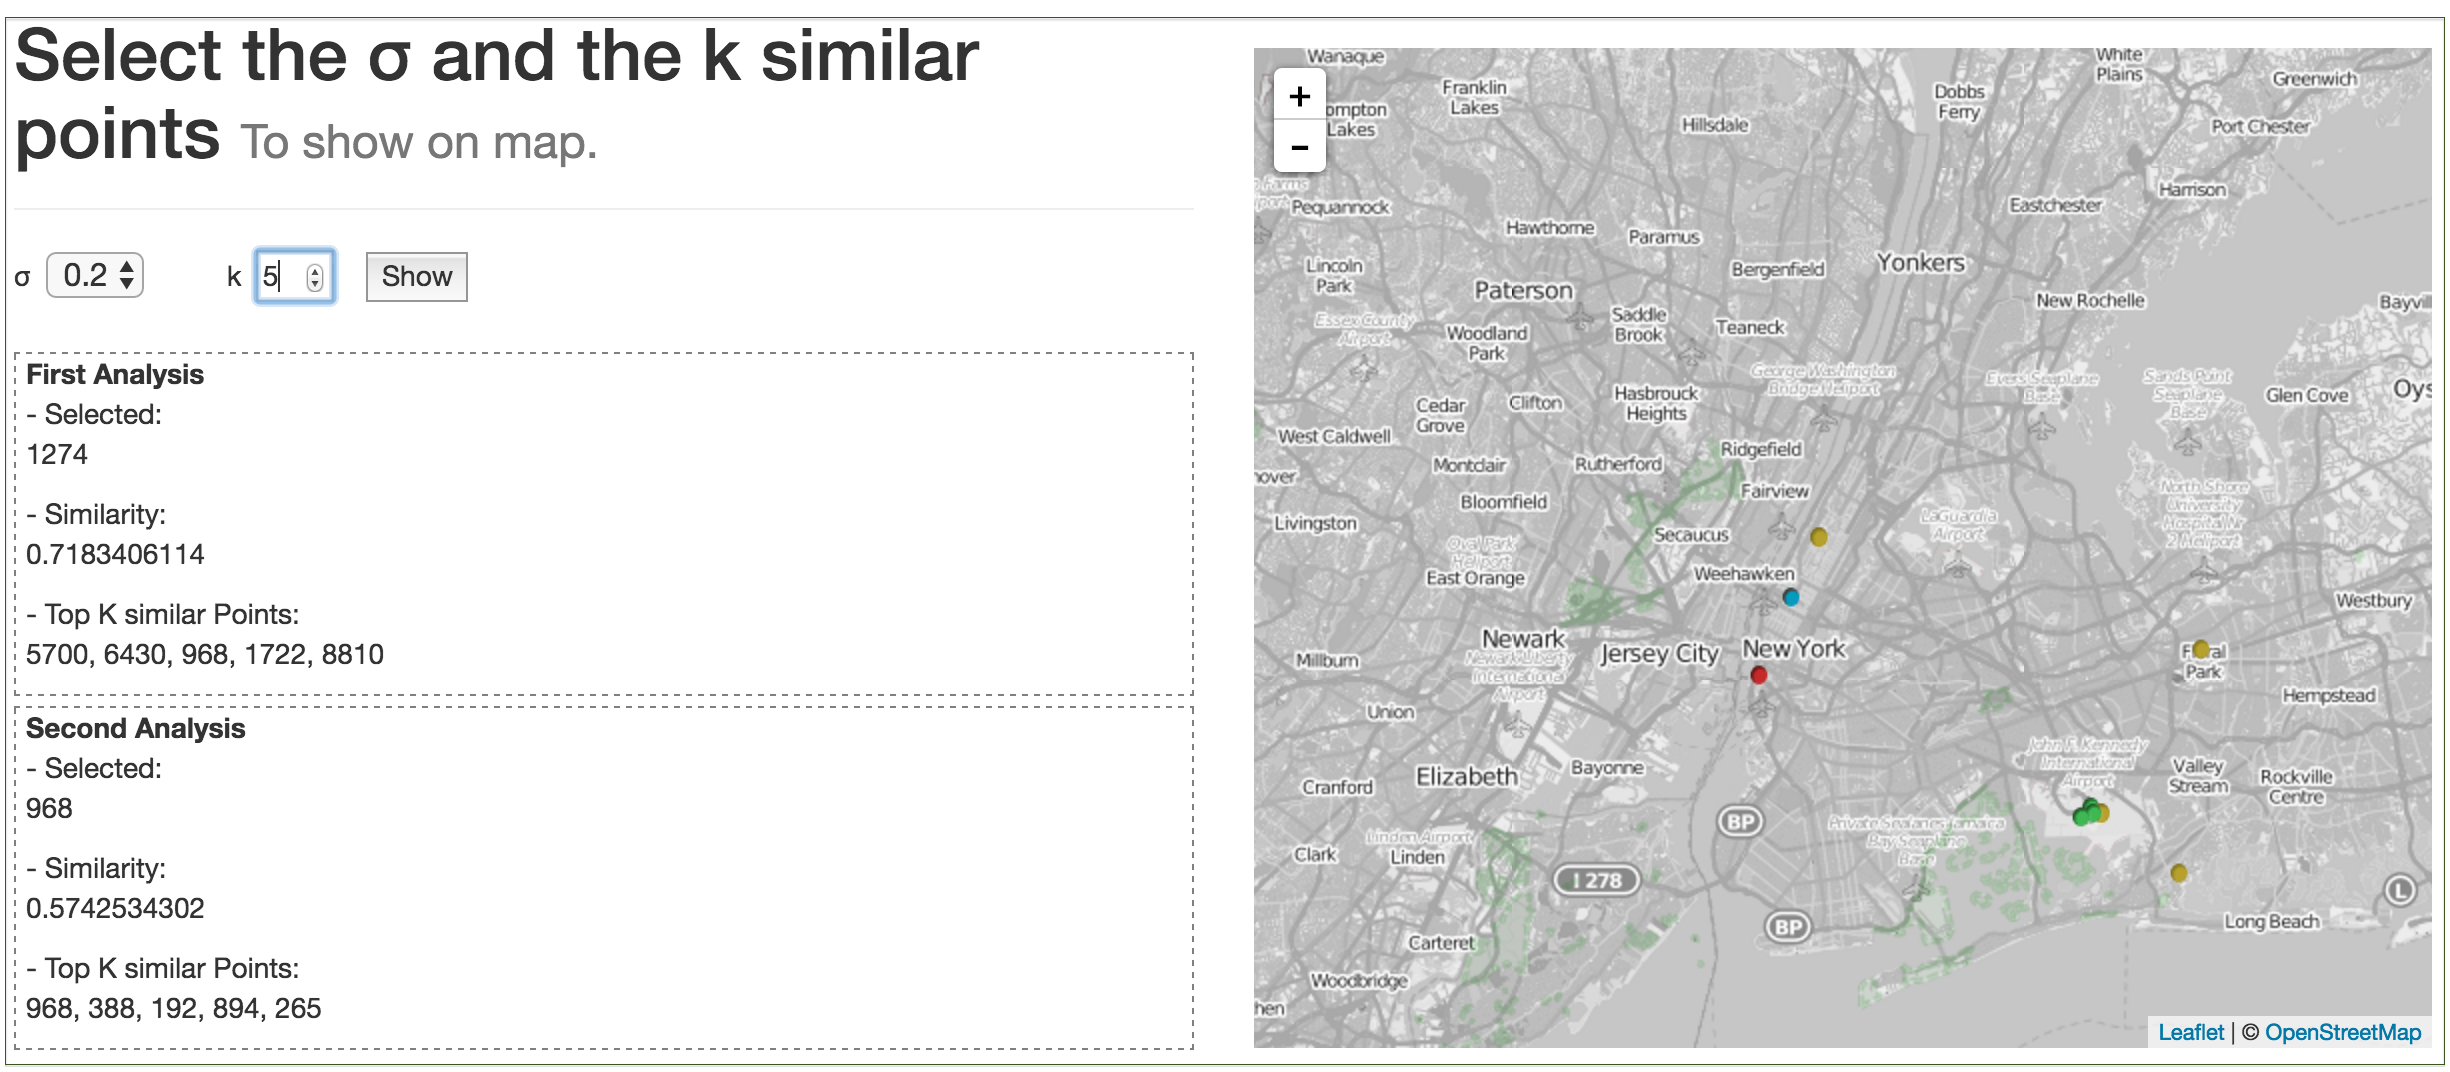
\includegraphics[width=\columnwidth]{figs/scenario.png}
\caption{Application of \framework\ on New York Taxi dataset}
\label{fig:app}
\end{figure}

% \vspace{5pt}
Consider Lucas, a data scientist whose task is to optimize New York taxi trips. Focusing on cab-idle locations, he wants to discover which neighborhoods work the best for which drivers to increase the overall availability. Also, he wants to discover how drivers should choose their next cab-idle station to be more available. Lucas employs \framework\ and follows a case-by-case inspection as his analysis methodology by analyzing and learning from historical data.

% coordinates of first point picked: lat, long: 40.757555, -73.988832. Point ID-1274, equivalent to 270 W 43rd St, New York, NY 10036, EUA. Next to Times Square.
% coordinates of the second point: lat, long: 40.789358,-73.970172000000005. Point ID-968, equivalent to Columbus Avenue, New York, NY, EUA.
%  coordinates of the third point: lat, long: 40.717531999999999,-74.010260000000002. Point ID-192, equivalent to 183 Duane Street, New York, NY 10013, EUA
He begins the analysis by selecting a point from the most crowded region in New York, i.e., Times Square. The point depicts a drop-off at {\em 270 West 43rd Street} on January 9, 2014 at 10PM (Figure \ref{fig:app}, \textit{blue point}). {\sc Highlighter} then provides $5$ relevant points to the selected point (Figure \ref{fig:app}, \textit{yellow points}).
% These highlights show similar points to the selection in other neighborhoods of the region.
Among 5 highlighted points, Lucas selects the 3rd one, i.e., a pick-up at {\em Columbus Avenue} near Central Park occurred approximately at the same time of the first selection (Figure \ref{fig:app}, \textit{yellow point} next to the \textit{blue point}). This pick-up has a potential to enchain with the first choice (i.e., a drop-off) to engage the driver in a larger distance.

In the next step, {\sc Highlighter} shows 5 other points relevant to the new selection. Lucas looks for a good drop-off point which is in a neighborhood of the previous selection as the cab-idle station (Figure \ref{fig:app}, \textit{green points}). Lucas selects the second highlighted point at {\em 183 Duane Street} at 10:20PM as other highlights are around airport and train stations which have less taxi requests in the afternoon (Figure \ref{fig:app},  \textit{red point}\footnote{\textit{This point is originally presented as a green point. We show it as a red point to highlight the final result.}}). This selection contributes to the heavy cab request in Manhattan island at that time of the day. 

% The result of similarity for all two executions of the algorithm for the Lucas problem, considering $k = 5$ and $\sigma = 0.2$, was approximately, \textit{0.72}.